\subsection{Dise\~no de m\'odulos de hardware del robot para pruebas de integraci\'on}
    %Parrafo 1
    En esta secci\'on se detalla el dise\~no de los m\'odulos de hardware del robot que hemos
        desarrollado para el Trabajo Terminal. El objetivo principal es asegurar una integraci\'on
        eficiente entre los diferentes componentes, permitiendo as\'i la realizaci\'on de pruebas
        de integraci\'on efectivas. La modularidad del dise\~no facilita tanto el desarrollo como el
        mantenimiento del sistema, as\'i como tambi\'en la sustituci\'on de algunos componentes,
        esto nos permite aislar y solucionar problemas de manera aislada.
    \vskip 0.5cm
    %Parrafo 2
    Nuestro robot desarrollado consta de cuatro m\'odulos principales: actuadores,
        sensores, unidad de control y m\'odulo de visualizaci\'on. Cada uno de estos m\'odulos
        cumple una funci\'on especifica que permite al robot moverse, detectar obst\'aculos, y
        seguir rutas predefinidas.
    \vskip 0.5cm
    %Figura 1
    \begin{figure}[htbp]
        \centering
        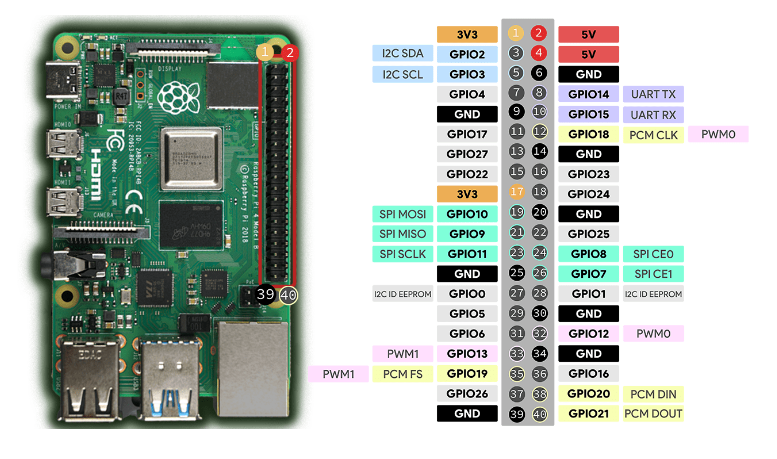
\includegraphics[width=0.5\textwidth]{./images/Pruebas/robot/robot01.png}
        \caption{Dise\~no de los pines de configuracion de los m\'odulos de hardware del robot.}
        \label{fig:robot}
    \end{figure}

    \subsubsection{M\'odulo de actuadores (Motores)} % (fold)
    \label{ssub:modact}
    El robot est\'a equipado por cuatro motores a pasos Nema 23, controlados a trav\'es de
        un controlador driver espec\'ifico para motores a pasos. Estos motores son
        responsables del movimiento del robot en las direcciones deseadas, permitiendo giros,
        avances y retrocesos mediante la manipulaci\'on precisa de los pines de control PWM y
        de direcci\'on.
    \vskip 0.5cm
    Los motores Nema 23 fueron elegidos debido a su precisi\'on en el posicionamiento y
        su capacidad para generar el torque necesario para mover la estructura del robot, que
        est\'a construida con perfiles de aluminio y ruedas omnidireccionales.
    \vskip 0.5cm
    % tabla 1
    \begin{longtable}{|c|c|c|c|}
        \hline
        \rowcolor{gray}
        \textbf{Producto} & \textbf{Descripci\'on} & \textbf{Piezas} \\
        \hline
        Motor a pasos Nema 23 & Motor a pasos Nema 23 con placa frontal & 4  \\
        Controlador de motores a pasos & Controlador de motores a pasos TB6600 & 4  \\
        Rueda omnidireccional & Rueda omnidireccional de 6 in & 4  \\
        \hline
        \caption{Especificaciones de los motores a pasos Nema 23.}
        \label{tab:motor}
    \end{longtable}
    \vskip 0.5cm
    Los motores est\'an conectados a los pines GPIO de la Raspberry Pi 4 B mediante un
        controlador de moteres. El sistema de control utiliza se\~nales PWM para regular la
        velocidad de los motores, y se\~nales de direcci\'on para controlar el sentido de giro.
    \vskip 0.5cm
    Elegimos los Motores Nema 23 debido a su precisi\'on y capacidad de generar torque
        necesario para mover el robot con su estructura de aluminio y ruedas
        omnidireccionales. Su tama\~no y especificaciones son ideales para aplicaciones que
        requieren alta precisi\'on en el movimiento.
    \vskip 0.5cm
    La incorporaci\'on de ruedas omnidireccionales de 6 pulgadas permite al robot realizar
        movimientos en varias direcciones sin necesidad de girar su estructura por completo.
        Esto optimiza la maniobrabilidad en entornos reducidos
    \vskip 0.5cm
    Finalmente elegimos los controladores a pasos por que estos son capaces de manejar
        la corriente y el voltaje necesario para los motores Nema 23, permitiendo un control
        preciso mediante se\~nales PWM generadas desde la unidad de control.
    \vskip 0.5cm
    % subsubsection  (end)
    \subsubsection{M\'odulo de sensores (LiDAR)} % (fold)
    \label{ssub:modsen}
    El robot est\'a equipado por un sensor YLiDAR 2XL, que permite realizar un escaneo de
        360° del entorno para detectar obst\'aculos y mapear el \'area de operaci\'on del robot. La
        elecci\'on de este sensor se debe a su capacidad para medir distancias con alta
        precisi\'on y su adecuado rango de operaci\'on, lo que lo convierte en una opci\'on ideal
        para la navegaci\'on aut\'onoma en tiempo real.
        El sensor se conecta a la unidad de control mediante un puerto USB tipo A.
    \vskip 0.5cm
    El sensor se conecta a la unidad de control mediante un puerto USB tipo A.
    \vskip 0.5cm
    El sensor de distancia se eligi\'o por su capacidad de ofrecer un rango de detecci\'on de
        8 metros de di\'ametro y su alta precisi\'on en el mapeo de entornos. Su \'angulo de
        escaneo de 360° permite que el robot detecte obst\'aculos en cualquier direcci\'on.
    \vskip 0.5cm
    Esta subsecci\'on no tiene un esquema de conexi\'on por que simplemente se conecta
        por USB tipo A.
    \vskip 0.5cm
    \subsubsection{Unidad de control (Raspberry Pi 4 B)} % (fold)
    \label{ssub:modcon}
    La unidad de Control es el cerebro del robot, responsable de gestionar y coordinar
        todos los m\'odulos de hardware, incluyendo los actuadores y los sensores. En este
        proyecto, se utiliza una Raspberry Pi 4 B, que ofrece la capacidad de procesamiento y
        la conectividad necesarias para integrar los diferentes componentes del sistema.
    \vskip 0.5cm
    La Raspberry Pi controla los motores mediante GPIO, recibe los datos del LiDAR a
        trav\'es del puerto UART, y adem\'as se encarga de la visualizaci\'on de la informaci\'on
        mediante una pantalla conectada o mediante el protocolo VNC.
    \vskip 0.5cm
    El dise\~no del m\'odulo de control se basa en la capacidad de la Raspberry Pi de gestionar
        m\'ultiples tareas simult\'aneamente, coordinando el movimiento del robot, la recepci\'on
        de datos de sensores, y la visualizaci\'on de la informaci\'on en una pantalla conectada.
    \vskip 0.5cm
    Se eligi\'o la Raspberry Pi 4 B debido a su capacidad para manejar m\'ultiples interfaces
        de comunicaci\'on (GPIO, UART) y su potencia de procesamiento, lo cual es crucial para
        la gesti\'on de m\'ultiples m\'odulos de hardware en tiempo real.
    \vskip 0.5cm
    \subsubsection{M\'odulo de visualizaci\'on} % (fold)
    \label{ssub:modvis}
    El modulo de visualizaci\'on permite monitorizar el entorno y la posici\'on del robot en
        tiempo real. Para ello, se utiliza una c\'amara de visi\'on nocturna conectada a la
        Raspberry Pi y un sistema de visualizaci\'on que integra los datos del sensor LiDAR en
        un mapa gr\'afico. La visualizaci\'on se realiza mediante una interfaz grafica que muestra
        tanto la imagen capturada por la c\'amara como el mapa generado por los datos del
        LiDAR.
    \vskip 0.5cm
    Elegimos una c\'amara infrarroja nocturna de 5MP para capturar video del entorno y
        verlo en la interfaz gr\'afica.
    \vskip 0.5cm
    El m\'odulo de visualizaci\'on est\'a dise\~nado para combinar la salida de la c\'amara con la
        representaci\'on gr\'afica de los datos del LiDAR, lo que facilita el monitoreo del entorno
        en tiempo real y la toma de decisiones basadas en la informaci\'on recopilada.
    \vskip 0.5cm
    La c\'amara infrarroja nocturna se eligi\'o por su capacidad para capturar im\'agenes de alta
        calidad en condiciones de poca luz, lo que permite al robot operar en entornos con
        iluminaci\'on deficiente.
    \vskip 0.5cm
    \subsubsection{Pruebas de integraci\'on} % (fold)
    \label{ssub:pruebas}
    Como parte del proceso de validaci\'on de los m\'odulos de hardware, se han planificado
        pruebas de integraci\'on cuyo objetivo ser\'a asegurar que todos los m\'odulos (actuadores,
        sensores, unidad de control y visualizaci\'on) funcionen de manera conjunta y
        coordinada. Estas pruebas estar\'an dise\~nadas para verificar que los m\'odulos puedan
        interactuar de forma efectiva en diversos escenarios, garantizando que el robot cumpla
        con los requisitos de funcionamiento aut\'onomo.
    \vskip 0.5cm
    Las pruebas de integraci\'on se dividir\'an en varias fases, las cuales ser\'an las siguientes:
    \begin{enumerate}
        \item Prueba de Conectividad entre m\'odulos
        \begin{itemize}
            \item Objetivo: Verificar que los m\'odulos de hardware se pueden comunicar
                entre s\'i de manera efectiva.
            \item Pasos:
                \begin{enumerate}
                    \item Configurar la conexi\'on UART entre la Raspberry Pi 4 B y el LiDAR YLIDAR 2XL.
                    \item Verificar la comunicaci\'on entre la Raspberry Pi 4 B y los motores a trav\'es de los pines GPIO (se\~nales PWM y direcci\'on).
                    \item Comprobar la conexi\'on de la c\'amara a la Raspberry Pi 4B.
                \end{enumerate}
            \item M\'etrica de \'exito: El tiempo de respuesta entre la se\~nal enviada desde la Raspberry Pi 4 B y la 
                recepci\'on de datos en los actuadores o sensores debe de ser menor a 100 ms.
            \item Criterio de \'exito: La conexi\'on entre los m\'odulos debe mantenerse
                estable durante al menos 1 hora de operaci\'on continua, sin p\'erdida de
                datos ni interrupciones.
        \end{itemize}
        \item Pruebas de movilidad y control de actuadores
        \begin{itemize}
            \item Objetivo: Evaluar la capacidad del robot para ejecutar movimientos b\'asicos
                (avance, retroceso, giros) de manera precisa y controlada.
            \item Pasos:
                \begin{enumerate}
                    \item Enviar se\~nales desde la unidad de control a los motores para probar el avance, retroceso y giros.
                    \item Ajustes la frecuencia PWM para probar diferentes velocidades de movimiento.
                    \item Medir la precisi\'on del moviento en distacias cortas y largas.
                \end{enumerate}
            \item M\'etrica de \'exito: Desviaci\'on m\'axima de 5cm en distancias cortas y de 10 cm en distancias largas.
            \item Criterios de \'exito: Los motores deben responder en menos de 500 ms
                tras recibir las se\~nales de control y realizar los movimientos sin errores.
        \end{itemize}
        \item Pruebas de detecci\'on de obst\'aculos
        \begin{itemize}
            \item Objetivo: Verificar la capacidad del robot para detectar obst\'aculos en su
                entorno y reaccionar de manera adecuada para evitar colisiones.
            \item Pasos:
                \begin{enumerate}
                    \item Realizar un escaneo completo del entorno con el sensor LiDAR.
                    \item Analizar los datos del LiDAR para identificar obst\'aculos y calcular
                        las distancias de seguridad.
                    \item Enviar se\~nales de control a los motores para evitar los obst\'aculos
                        detectados.
                \end{enumerate}
            \item M\'etrica de \'exito: El robot debe ser capaz de detectar obst\'aculos a una
                distancia m\'inima de 15cm y reaccionar de manera efectiva para evitar
                colisiones.
            \item Criterios de \'exito: El robot debe ser capaz de evitar obst\'aculos en un
                entorno cerrado con una tasa de \'exito del 90\%.
        \end{itemize}
        \item Pruebas de Seguimiento de Rutas Predefinidas
        \begin{itemize}
            \item Objetivo: Evaluar la capacidad del robot para seguir rutas predise\~nadas,
            ajustando su trayectoria en respuesta a cambios en el entorno.
            \item Pasos:
                \begin{enumerate}
                    \item Trazar una ruta en un entorno controlado.
                    \item Activar el sistema de seguimiento de rutas del robot.
                    \item Introducir obst\'aculos inesperados y verificar que el robot ajuste
                        su trayectoria sin desviarse significativamente.
                \end{enumerate}
            \item M\'etrica de \'exito: El robot debe seguir la ruta trazada con una desviaci\'on
                m\'axima de 10 cm en trayectorias rectas y de 15 cm en giros.
            \item Criterio de \'exito: El robot debe ajustar su trayectoria en menos de 1
                segundo tras detectar un cambio en el entorno.
        \end{itemize}
        \item Pruebas de Visualizaci\'on en Tiempo Real
        \begin{itemize}
            \item Objetivo: Verificar que la interfaz gr\'afica del robot muestra la
                informaci\'on del entorno y la posici\'on del robot en tiempo real.
            \item Pasos:
                \begin{enumerate}
                    \item Iniciar la c\'amara de visi\'on nocturna y el sensor LiDAR.
                    \item Mostrar la imagen capturada por la c\'amara y el mapa generado por
                        el LiDAR en la interfaz gr\'afica.
                    \item Verificar que la informaci\'on se actualiza en tiempo real y que el
                        robot se representa correctamente en el mapa.
                \end{enumerate}
            \item M\'etrica de \'exito: La interfaz gr\'afica debe mostrar la informaci\'on del
                entorno y la posici\'on del robot con una latencia m\'axima de 500 ms.
            \item Criterio de \'exito: La interfaz gr\'afica debe actualizarse en tiempo real y
                mostrar la informaci\'on del entorno y la posici\'on del robot de manera precisa.
        \end{itemize}
    \end{enumerate}